\section{MobiScope Overview}
\label{sec:platform}

% This section describes the goals for our monitoring approach, and how
% \platname achieves these goals using proxying.  We show that our
% approach imposes reasonable overheads, and we describe how our
% IRB-approved study protects user privacy.

% \subsection{Goals}
% \label{sec:goals}
% Our primary goal is \emph{to monitor all the Internet traffic from
%   mobile devices regardless of the operating system, wireless access
%   technology, and the ISPs used by the mobile device}.  To achieve
% this goal, we identify the following desirable properties for a
% measurement platform:
% \begin{packedenumerate}
% \item \emph{Portable.} Our approach should work on all major device
%   OSes without requiring support from carriers or ISPs.
% \item \emph{Pervasive.} We should be able to measure traffic
%   regardless of the location, access technology, and ISPs used by
%   mobile devices.
% \item \emph{Passive.} We wish to understand the network traffic
%   naturally generated by users and their devices, requiring passive
%   monitoring.
% \item \emph{Deployable.} We want a low barrier to entry to facilitate
%   large-scale adoption with minimal impact on the user
%   experience. \tbd{We need to say easy to controlled perform
%     experiments}
% \end{packedenumerate}

In this section, we present the \platname{} plateform whose goal is
\emph{to monitor all the Internet traffic from and to mobile devices}
with the following constraints.
\begin{packedenumerate}
\item \emph{OS agnostic.} We want to monitor traffic independently of
  the OS run by the monitored device. In particular, we do not want to
  develop OS specific applications, or to root or jailbreak the phone.
\item \emph{ISP agnostic.} We want to monitor traffic without any
  support from ISPs and cellular providers.
\item \emph{Access technology agnostic.} We want to monitor traffic
  whatever the access technology used by the mobile device (Wifi, GSM,
  CDMA, UMTS, LTE, etc.)
\item \emph{Encryption agnostic.} We want to monitor traffic both in
  clear and encrypted.
\item \emph{Flow modification.} We want to not only monitor, but
  also possibly modify data packets in order to experiment. This makes
  \platname{} both a passive monitoring and an experimental
  platform. 
\item \emph{Single machine.} We want \platname{} to fit on a
  single machine to facilitate its installation and deployment. 
 \end{packedenumerate}    

At the time of the camera ready version, we will make the \platname{}
software publicly available. 


\subsection{MobiScope Design}

% We now describe how we achieve these goals using proxying.
% Specifically, we use two approaches to proxy mobile traffic: secure
% proxying via virtual private networks (VPNs) and insecure transparent
% proxying.  These two approaches allow us to measure traffic with and
% without carrier interposition, respectively.

% \subsubsection{VPN Proxying}
% \label{sec:platform-vpn}

In order to monitor all Internet traffic from and to mobile devices
with the constraints we described, we designed the \platname{} plaform
on a VPN infrastructure. By instrumenting the VPN server that
mobile devices are using, we can monitor all the Internet traffic going
through the VPN tunnels. But, using a VPN infrastructure raises three
important questions. i) How ubiquitous is the VPN technology on mobile
devices?  ii) How to monitor traffic on \platname{}? iii) How to
modify traffic on \platname? We explore in the following these three key questions.

\subsubsection{VPN Technology on Mobile Devices}
\label{sec:vpn-tech-mobile-device}
The VPN technology is widely supported on the most popular mobile
OSes. Indeed, Android, BlackBerry, Bada, and iOS all support VPNs,
primarily to satisfy their enterprise clients that use VPNs to
securely connect to their enterprise networks. Also, the VPN
technology on mobile devices encapsulates all the data traffic---both
Wi-Fi and cellular. Consequently, it is possible to reach our three
first design goals: OS, ISP, and access technology agnostic.

However, to capture all Internet traffic from and to a mobile device,
a VPN must always be enabled. Currently, all iOS devices (version 3.0
and above) support a feature called \textit{VPN On-Demand}.  VPN
On-Demand forces the iOS device to use VPN tunnels when connecting to
a specified set of domains, and we configured it to be enabled for all
Internet domains. Android version 4.2 and above support an
\textit{Always On VPN} connection that is always enabled for all data
traffic, and Android version 4.0 and above provide an API that allows
applications to manage VPN tunnels. We implemented an application that
uses this API in order to provide the always on functionality for
Android 4.0 and 4.1.

In addition, to facilitate the creation of certificates to configure
the VPN tunnels between the mobile devices and the \platname{}
platform, we created our own \platname{} root certificate that is used
to sign all subsequent certificates issues to mobile devices that want
to use the \platname{} platform. 

In summary, the VPN technology is available out-of-the-box for the
latest versions of the most popular mobile OSes. From the server side,
that is on the \platname{} platform, we use
\textit{Strongswan}~\cite{strongswan}, an open source software used to
manage VPN tunnels. Strongswan supports the required protocols and
encryption algorithms required by iOS and Android, in particullar
IPsec for the encryption of IP datagrams and IKEv1 and
IKEv2~\cite{rfc5996} for authentication and key negotiation.


% The use IPsec by mobile devices for pervasive VPN tunnels limited our
% choice of VPN daemons to manage VPN tunnels on our proxying server.
% Though VPN daemons manage tunnels created using protocols such as PPTP
% and L2TP, the ``VPN On-Demand'' feature of iOS is available only for
% VPN tunnels that use IPsec.  To the best of our knowledge, the only
% publicly available VPN daemon that uses IPsec in Linux \emph{without
%   any kernel modifications} is Strongswan~\cite{strongswan}.
% Strongswan also supports the faster IKEv2~\cite{rfc5996} based
% authentication which is supported by Android devices.

% \subsubsection{Advantages and Drawbacks of VPNs}
% \label{sec:advant-drawback-vpn}



\subsubsection{Monitoring Traffic on MobiScope}
\label{sec:monit-traff-mobiscope}

Surprisingly, monitoring traffic on \platname{} is particularly
involved. When we monitor traffic on \platname, we need to dump
all traffic between the mobile devices and the Internet, and we need to
associate the dumped traffic to the right mobile device and Webservice. The
former is easy using a \textit{tcpdump} process, but the later is more
complex. To explain this complexity, we first need to explain how
packets are processed on \platname. 


\begin{figure}
\begin{center}
  \subfloat[Packet from mobile device. \emph{Tcpdump can capture
    packets at step (2)~d~$\rightarrow$~m, (4)~v~$\rightarrow$~w, and
    (7)~m~$\rightarrow$~w.}]{\label{fig:packet-monitor-a}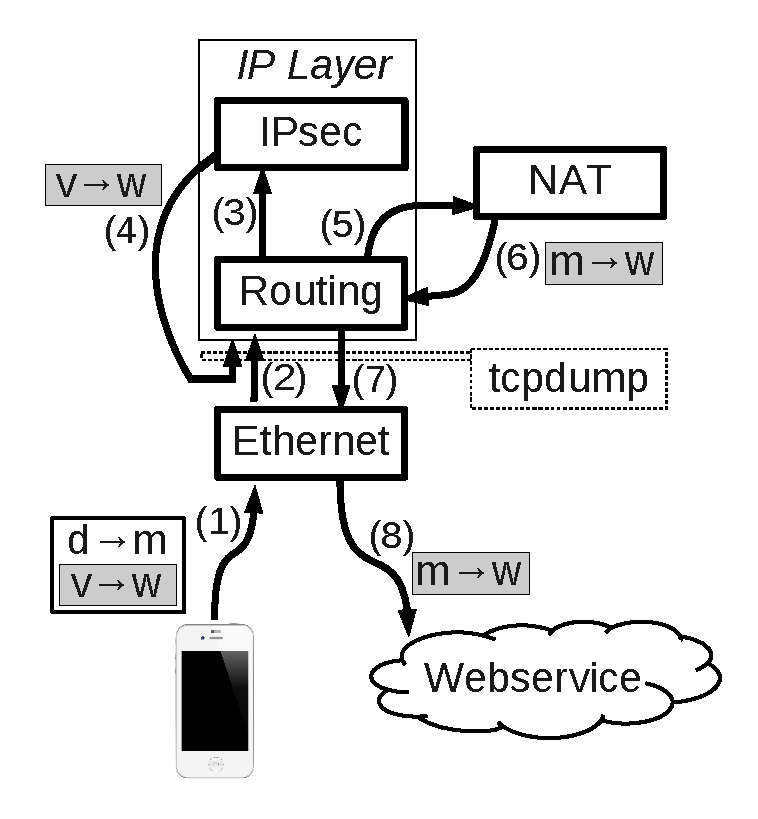
\includegraphics[width=0.47\columnwidth]{figures/packet-monitoring-a.pdf}}
  \hspace{0.05\columnwidth} \subfloat[Packet to mobile
  device. \emph{Tcpdump can capture packets at step
    (2)~w~$\rightarrow$~m and (7)~m~$\rightarrow$~d, however it is
    cannot log the packet
    w~$\rightarrow$~v.}]{\label{fig:packet-monitor-b}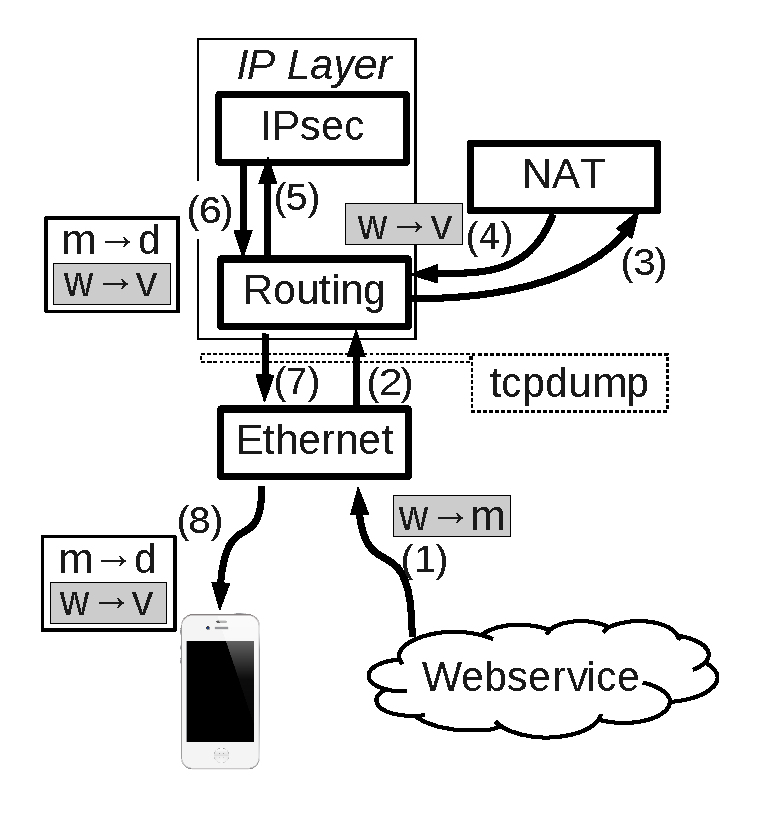
\includegraphics[width=0.47\columnwidth]{figures/packet-monitoring-b.pdf}}
  \newline \subfloat[Packet from mobile device. \emph{Tcpdump
    monitoring packets on the tun device can capture packets at step
    (5)~v~$\rightarrow$~w, and
    (6)~v'~$\rightarrow$~w.}]{\label{fig:packet-monitor-c}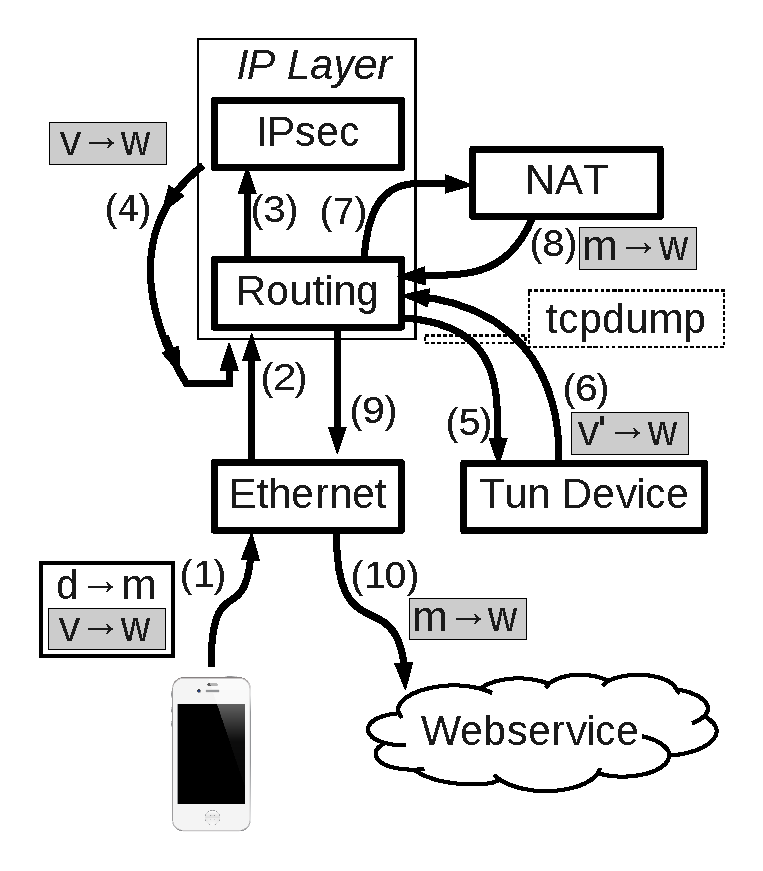
\includegraphics[width=0.47\columnwidth]{figures/packet-monitoring-c.pdf}}
  \hspace{0.05\columnwidth} \subfloat[Packet to mobile
  device. \emph{Tcpdump monitoring packets on the tun device can
    capture packets at step (5)~w~$\rightarrow$~v', and
    (6)~w~$\rightarrow$~v.}]{\label{fig:packet-monitor-d}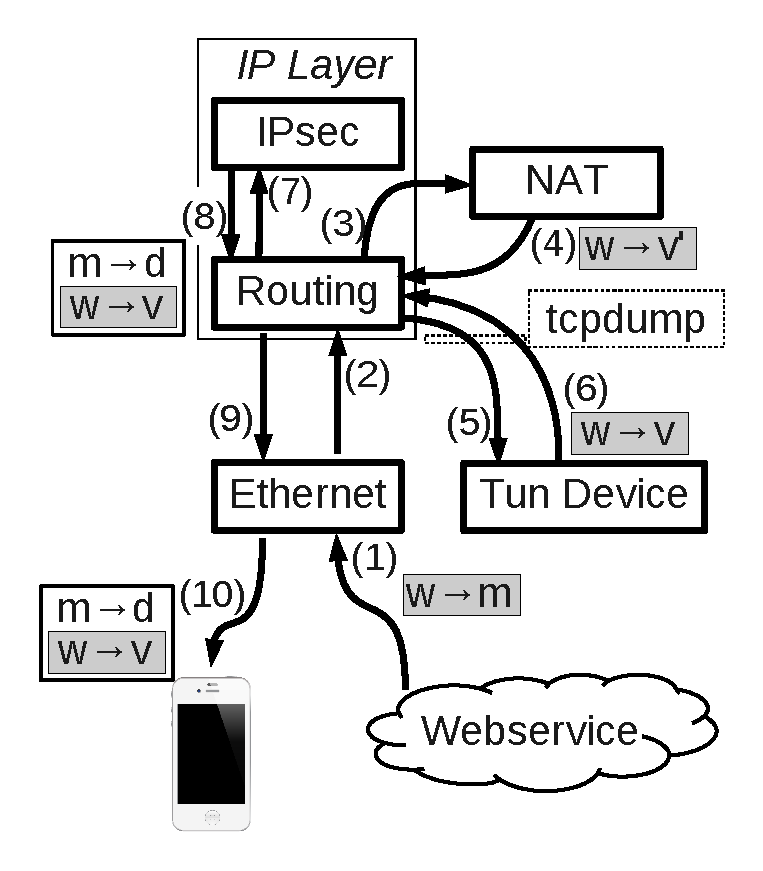
\includegraphics[width=0.47\columnwidth]{figures/packet-monitoring-d.pdf}}
  \newline
\begin{small}
\begin{tabular}{|c|p{0.8\columnwidth}|}
\hline
Symbol & Description \tabularnewline
\hline
d & IP address of the mobile device assigned by its ISP. \tabularnewline
m & IP address of the \platname server. \tabularnewline
w & IP address of the server providing the Webservice. \tabularnewline
(i) & The i-th step of packet processing. \tabularnewline
\fbox{a $\rightarrow$ b} & Packet with source IP \emph{a} and destination IP \emph{b}. \tabularnewline
v & IP address of the mobile device in the VPN tunnel. \tabularnewline
v' & Temporary IP address of the mobile device used to send the packet
to the TUN device. \tabularnewline

\hline
\end{tabular}
\end{small}
\end{center}
\caption{Packet monitoring in the \platname{} box.}
\label{fig:packet-monitoring}
\end{figure}

Figure~\ref{fig:packet-monitor-a} shows the processing on \platname{}
of packets sent from a mobile device to the Internet. At step (1),
(2), and (3) the encrypted datagram (in gray) goes up the layers, this
datagram is encapsulated in a regular IP datagram sent from the device
(address \emph{d}) to the \platname{} box (address \emph{m}). The
IPsec layer decrypts at step (3) the datagram whose source IP address
is the private address of the mobile device in the VPN tunnel (address
\emph{v}) and the destination is the IP address of the destination
Webservice (address \emph{w}). In order to send this datagram in the
Internet, the NAT must convert in step (5) the private IP address
\emph{v} to the public IP address \emph{m} of the \platname{}
box. Then this packet is sent in the Internet. As the tcpdump process
runs just above the Ethernet layer, it dumps packets at step (2), (4),
and (7). In addition, we also dump the NAT translation
table. To associate packets to a device and a Webservice,
we only need the packet captured at step (4) that associates the
packet to the private address \emph{v} of the device in the VPN tunnel
and the Webservice (address \emph{w}), and the NAT translation table
that gives the mapping between the device in the VPN tunnel (address
\emph{v}) and the public IP address \emph{d} of the mobile device.

However, in the reverse direction, when packets flows from the
Internet to the mobile device, it is no more possible to associate a
mobile device to the packets, see
Figure~\ref{fig:packet-monitor-b}. Indeed, from the dumped packets at
step (2) and (7), we know that a packet in sent by the Webservice to
the \platname{} box (step (2)), but then this packet is encapsulated
at the IPsec layer, and the address resolution is performed by the NAT
without any dump. So, when we see the datagram at step(7), we have no
way to know which encrypted packet is encapsulated. We need to dump
the packet at step (4), but we have no access to it. One way would be
to run the NAT on a separate box, and to dump traffic from that box,
but it would require two different boxes. Instead, we propose a
solution that allows to dump the packet from \emph{w} to \emph{v} from
a single box, which we describe in the following. 

Our solution is to force the packets from \emph{w} to \emph{v} to make
a loop on a TUN device, and to dump these packets at the TUN device,
see Figure~\ref{fig:packet-monitor-d}. Indeed, when a packet is
received from the Internet is goes up the layers up to the NAT at step
(3). At that point, the NAT resolve the public address of the
\platname{} box \emph{m} to the address of the device in the VPN
tunnel \emph{v}. In the NAT all addresses in the VPN tunnel are class
A private addresses using only 23 bits out of 24. The 24th bit has a
specific role. By default it is set to 0, but we modified the NAT so
that when it receives a packet that resolve to \emph{v}, it changes it
to \emph{v'} that only differ from \emph{v} by the 24th bit that is
set to 1. The only one reason to make this conversation is to send all
packets whose destination is \emph{v} to the TUN device, by creating a
specific forwarding rule that forwards all packet with a \emph{v'}
destination address (a class A private address with the 24th bit set
to 1) to the TUN device, step (5). Then, we implement a process at the
TUN device whose only one goal is to change the destination address
from \emph{v'} to \emph{v}, and to sends back the packet to the IP
layer, step (6). Then the packet follows the path of a regular packet
in a VPN tunnel. 

When a packet is received from the mobile device, we perform a similar
process that is described in Figure~\ref{fig:packet-monitor-c}. 

In summary, exploiting the notion of TUN device, we are now able to
dump all Internet traffic from and to a mobile device connected to the
\platname{} platform from a single machine, and to associate this
traffic to corresponding mobile devices and Web services. 



% %start the discussion of the technical details. TO REWRITE
% The IPsec implementation in the Linux kernel is not suitable to
% traffic monitoring when the server running the VPN daemon is used to
% proxy Internet traffic.  A VPN Proxy, apart from serving VPN tunnels,
% relies on NAT to proxy Internet traffic.  When a mobile device
% establishes a VPN tunnel, the VPN server assigns it assigned a private
% IP address.  The mobile device therefore has two IP addresses, a
% private address assigned by the VPN server, and a public IP address
% assigned by the service provider.  The public IP address is used only
% to communicate with the VPN server while all other communication uses
% the private IP address.  Therefore all the traffic that would have
% used the public IP address when the VPN tunnel was not present, now
% uses the private IP address.  These packets that use the private IP
% are encapsulated and encrypted using IPsec and sent to the VPN server.
% The VPN server decapsulates these packets before forwarding them.
% Before forwarding the packet, the VPN server must perform NAT because
% these private IP address cannot used in the Internet.  The use of NAT
% and IPsec implies that the forwarding each packet by the server is
% governed by two rules: one rule to enforce IPsec encryption and
% decryption of packets that contain the public IP of the mobile device,
% and the other that enforces NAT for packets with the private IP
% address.

% An association between the mobile device and a packet is possible only
% if the packet encapsulated within an IPsec packets is monitored in the
% clear.  However, the current implementation of NAT and IPsec makes
% this association of packets with the mobile devices non-trival.  A
% packet from the mobile device, encrypted using IPsec, needs to be
% decrypted before undergoing NAT.  As shown in
% \fref{fig:packet-monitoring-problem}, because the IPsec computations
% take place after the NAT computations, the kernel loops the packet
% back to the IP layer after decryption.  This looping allows the packet
% monitor to observe the IPsec packet before and after
% decryption\footnote{A similar operation takes place if the mobile
%   devices communicate with each other over P2P however we do not
%   discuss this scenario due to lack of space.}.  When multiple flows
% pass through the VPN server, the packet monitor can use the private IP
% address to associate the packets with the mobile device.  Once the NAT
% operation is performed the packet is forwarded via the network card.
% When the network card receives a packet intended for the mobile
% device, as shown in \fref{fig:packet-monitoring-problem}, the packet
% first undergoes NAT followed by IPsec encryption.  The encrypted
% packet is then sent to the mobile device.  Because the packet is not
% looped through the packet monitor before encryption, the packet
% monitor is not able to see the packet after NAT and before encrpytion.
% This implies without any modifications, any off the shelf packet
% monitor shall fail to associate the packets destined for mobile
% devices with the corresponding mobile device.

\subsubsection{Modifying Traffic on MobiScope}
\label{sec:modif-traffic-mobiscope}

\begin{figure}
\begin{center}
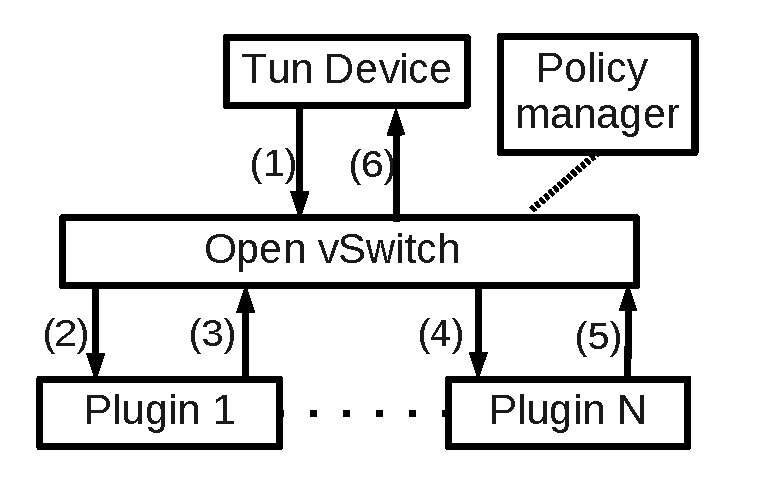
\includegraphics[width=0.8\columnwidth]{figures/packet-monitoring-plugin.pdf}
\end{center}
\caption{Plugin Infrastructure on \platname.}
\label{fig:packet-monitoring-solution}
\end{figure}

We described in section~\ref{sec:monit-traff-mobiscope}, how we can
monitor all Internet traffic on the \platname{} platform, using the
notion of TUN device. In that section, we explain here how we can use
this same notion of TUN device to build a powerful plugin
infrastructure enabling any traffic modification.

Figure~\ref{fig:packet-monitoring-solution} shows the plugin
infrastructure of \platname. When a packet is received at the TUN
device, it is sent to an open vSwitch~\cite{Openvswitch} process whose
goal is to define in which order each plugin will receive
packets. This order is configured by the policy manager. So packets
flow through each plugin, being processed at each plugin. 

Plugins can be used for many different purposes such as replaying
traffic, testing reliability to data corruption or delays, or
decrypting SSH traffic. In the following, we describe how easy it is
to perform SSH traffic decryption using the \platname{} plugin
infrastructure.

In order to perform SSH traffic decryption, we use a 
feature of the Squid proxy called SSL bumping\tbd{AR: give a
  reference}. This feature consists in performing a man-in-the-middle
attack. When the mobile device connects to a Web service, the squid
proxy impersonates the Web service using a forged certificate signed
with the root certificate of the \platname{} platform (see
Section~\ref{sec:vpn-tech-mobile-device}). Then the squid proxy
negotiate with the Web service a SSL session, impersonating a mobile
device. Using the traffic dumped by the tcpdump process as shown in
Figures~\ref{fig:packet-monitor-c} and \ref{fig:packet-monitor-d}, and
using the private key generated by the squid proxy to communicate with
the mobile device, we can decrypt all SSL traffic. We notice that when
traffic is not encrypted using SSL, the squid proxy simply acts as a
transparent proxy. 

Impersonating a Web service using a root certificate that is not
issued by a well known root authority might fail if the application on
the mobile device only allows certificate issued by well known
authorities. Surprisingly, this is rarely the case. Whereas the
Twitter application and the Firefox browser prevent SSL bumping by
validating the root certificate, Google Chrome, Safari, the Facebook
application, the Google+ application, the default mail clients, and
advertisement services do not check the validity of the root
certificate, thus the SSL bumping attack is possible. We will discuss
further this issue in Section~\ref{sec:classification}. 

% \begin{figure}
% \begin{center}
% \includegraphics[width=0.8\columnwidth]{figures/tun-device.pdf}
% \end{center}
% \caption{Tun-tap device to loop packets for packet monitoring.}
% \label{fig:packet-monitoring-solution}
% \end{figure}

% To monitor the packets that are encapsulated within IPsec packets we
% route the packets through a tun-tap device before encryption and after
% decryption.  As shown in \fref{fig:packet-monitoring-solution},

% \subsubsection{Transparent Proxy}
% \label{sec:platform-transparent-proxy}


\subsection{Feasibility}


\subsection{Limitation}
\platname {} has reached all the design goals, making this platform an
excellent choice to monitor traffic for mobile devices. However,
\platname{} has one limitation: because all the traffic between mobile
devices and \platname{} is encrypted, we cannot observe any traffic
modification made by ISPs. Indeed, ISPs that modify traffic (e.g., to insert
advertisements \tbd{AR: give a reference}) must perform deep packet
inspection, which is not possible when the traffic is encrypted.  In
this section, we assess to which extent this issue is a practical
limitation for \platname.


\tbd{AL: put tripwire experiments here to show that ISP traffic
  modification does not impact much Mobiscope. }

%%% Local Variables: 
%%% mode: latex
%%% TeX-master: "main.tex"
%%% End: 
